% Functional specification for ProfiSnort
\documentclass[listof=totoc,a4paper]{scrreprt}

\usepackage[german]{babel}
\usepackage[utf8]{inputenc}
\usepackage[T1]{fontenc}
\usepackage{ae}
\usepackage[bookmarks,bookmarksnumbered]{hyperref}
\usepackage{csquotes}
\usepackage{longtable}
\usepackage{enumitem, hyperref}
\usepackage{graphicx}

\usepackage{float}
\usepackage{verbatim}

\usepackage[ampersand]{easylist}
\usepackage{xcolor}

\usepackage[toc,acronym]{glossaries}
\makeglossaries

\setuptoc{toc}{totoc}

\usepackage{xparse}
\DeclareDocumentCommand{\newdualentry}{ O{} O{} m m m m } {
  \newglossaryentry{gls-#3}{name={#5},text={#5\glsadd{#3}},
    description={#6},#1
  }
  \makeglossaries
  \newacronym[see={[Glossary:]{gls-#3}},#2]{#3}{#4}{#5\glsadd{gls-#3}}
}

\renewcommand*{\glstextformat}[1]{\textcolor{black}{#1}}

\hypersetup{
	backref,
    colorlinks,
    linkcolor=[RGB]{0,153,84},
    citecolor={blue!40!black},
    urlcolor={blue!70!black},
    linktocpage=true
}

\makeatletter
\def\namedlabel#1#2{\begingroup
    #2%
    \def\@currentlabel{#2}%
    \phantomsection\label{#1}\endgroup
}
\makeatother

\newcounter{savepage}

\newcommand{\sppname}{spp\_profinet}
\newcommand{\programname}{TruffleHog}


\loadglsentries{../../global_tex_files/glossary}


\begin{document}

\title{\programname \ \& \sppname \ -- Entwurf}
\author{
    Brendl, Julian
    \texttt{julian.brendl@student.kit.edu}
    \and
    Diez, Maximilian
    \texttt{maximilian.diez@student.kit.edu}
    \and
    Giraud, Mark
    \texttt{mark.giraud@student.kit.edu}
    \and
    Hermes, Jan
    \texttt{jan.hermes@student.kit.edu}
    \and
    Höhler, Dimitri
    \texttt{dimitri.hoehler@student.kit.edu}
    \and
    Kiechle, Valentin
    \texttt{valentin.kiechle@student.kit.edu}
}

\titlehead{\includegraphics[width=150pt]{images/title.png}}

\maketitle

\pagenumbering{Roman}
\setcounter{page}{2}

\newpage
\tableofcontents
\newpage
\listoffigures

\printglossary[title=Abkürzungsverzeichnis,toctitle=Abkürzungsverzeichnis,type=acronym]

\clearpage
\setcounter{savepage}{\arabic{page}}
\pagenumbering{arabic}
\setcounter{page}{\thesavepage}

\chapter{Einleitung} 
Dieses Dokument dient der genaueren Beschreibung und Dokumentation des Entwurfs zum Visualisierungstool Trufflehog, dessen Hauptaufgabe die Darstellung des Netzwerkverkehrs eines ProfiNet-Systems ist. Des Weiteren wird der im IDS Snort eingebaute Präprozessor \sppname und die genaue Funktionsweise der Inter-Prozess-Kommunikation (im Folgenden IPC) zu Trufflehog genau erläutert.

Das Design von Trufflehog baut auf dem klassischen Model-View-Controller (im Folgenden MVC) auf und erweitert diesen Entwurf zu einem Model-View-Presenter mit zusätzlicher Funktionalität.

//hier MVC von Präsentation und ähnliches Bild zum aktuellen Entwurf einfügen//


\chapter{Architektur und Musterbeschreibung}
Im Groben gehalten funktioniert der Daten- und Befehlsfluss im Trufflehog-Entwurf wie im klassischen MVC, der Presenter aktiviert Services, welche das Model basierend auf dem empfangenen Netzwerkverkehr verändert und das View aktualisiert sich am Model. Da viele Threads im Programm parallel durchlaufen aber dennoch kommunizieren müssen, verlassen wir uns an einigen Stellen auf das \gls{observerpattern} mit einer Multi-Thread kompatiblen Datenstruktur.\newline
\newline


\section{\textbf{commands-Package:}}


Die Kernfunktionalität innerhalb des Programms stellt das \textbf{commands-Package}. Darin befinden sich sowohl die Hierarchie, vorhandene Datenstruktur als auch jede mögliche Command-Klasse und deren Interface. Vom Prinzip her vergleichbar mit Runnables.\newline

\begin{figure}[H]
  \centering
  \includegraphics[width=\textwidth]{../diagramimages/commands.png}
  \caption{\textbf{commands-Package}}
\end{figure}

Es gibt 2 Hauptarten von Commands, UserCommands für die Verwaltung der Benutzeroberflächenbefehle, und TruffleCommands für die Methodenaufrufe im Model-Graph, also die Hauptarbeit am Model. Die Commands machen außerdem den Hauptteil der Log-Datein und damit der Video-Funktion aus. Mehr dazu im service-Unterpackage datalogging.

    \subsection*{\textbf{commandQueue}}
    Die besagte Datenstruktur, welche beispielsweise der executor besitzt. Es sind ggf. mehrere tatsächliche Queues vorhanden, was einen Manager verlangt um nach dem Round-Robin-Prinzip faire Verteilung zu ermöglichen.


\section{\textbf{service-Package:}}


In unserem Entwurf haben wir uns außerdem dazu entschieden einzelne durchlaufende Arbeitsschritte in das \textbf{Service-Package} auszulagern.\newline

\begin{figure}[H]
  \centering
  \includegraphics[width=\textwidth]{../diagramimages/service.png}
  \caption{\textbf{service-Package}}
  \medskip
\end{figure}

    \subsection*{\textbf{truffleprocessor}}
    Der \textbf{truffleprocessor} ist die Empfangsstelle für die von uns in der \gls{ipc} benutzen Truffles. Außerdem erzeugt er die später verwendeten Commands und benachrichtigt als \gls{notifier}.
    
    \subsection*{\textbf{datalogging}}
    Das \textbf{datalogging} kümmert sich um die gesamte gewünschte Speicherung/Loggen und, falls implementiert, die Verfügbarkeit der Video-Daten. Es speichert sowohl regelmäßige Snapshots des gesamten Graphen, als auch einzelne Commands für eine Schrittweise Rückverfolgung des Ablaufes.
    
    \subsection*{\textbf{executor}}
    Der \textbf{executor} ist das Unterpackage, in welchem die Anwendung bzw. Ausführung der Commands stattfindet. Er ist ein \gls{listener} für Commands von sowohl dem view-Package als auch dem truffleprocessor.


\section{\textbf{presenter-Package:}}


Der \textbf{presenter} ist für den Aufbau von \gls{programname}, also das Initialisieren, Instanziieren und Referenzieren aller Programmelemente zuständig.

\begin{figure}[H]
  \centering
  \includegraphics[width=\textwidth]{../diagramimages/presenter.png}
  \caption{\textbf{presenter}}
\end{figure}

Er ist der erste Thread und erzeugt alle weiteren, zum Beispiel einen für jeden Service. Außerdem liest er aus einer Settings-Datei und stellt das Programm ein.
Das heisst er initialisiert bestimmte Attribute entsprechend. Danach erschöpft sich die Nützlichkeit des \textbf{presenter} bis zu einem neuen Programmstart.


\section{\textbf{util-Package:}}


Unsere Variante des \gls{observerpattern}s.

\begin{figure}[H]
  \centering
  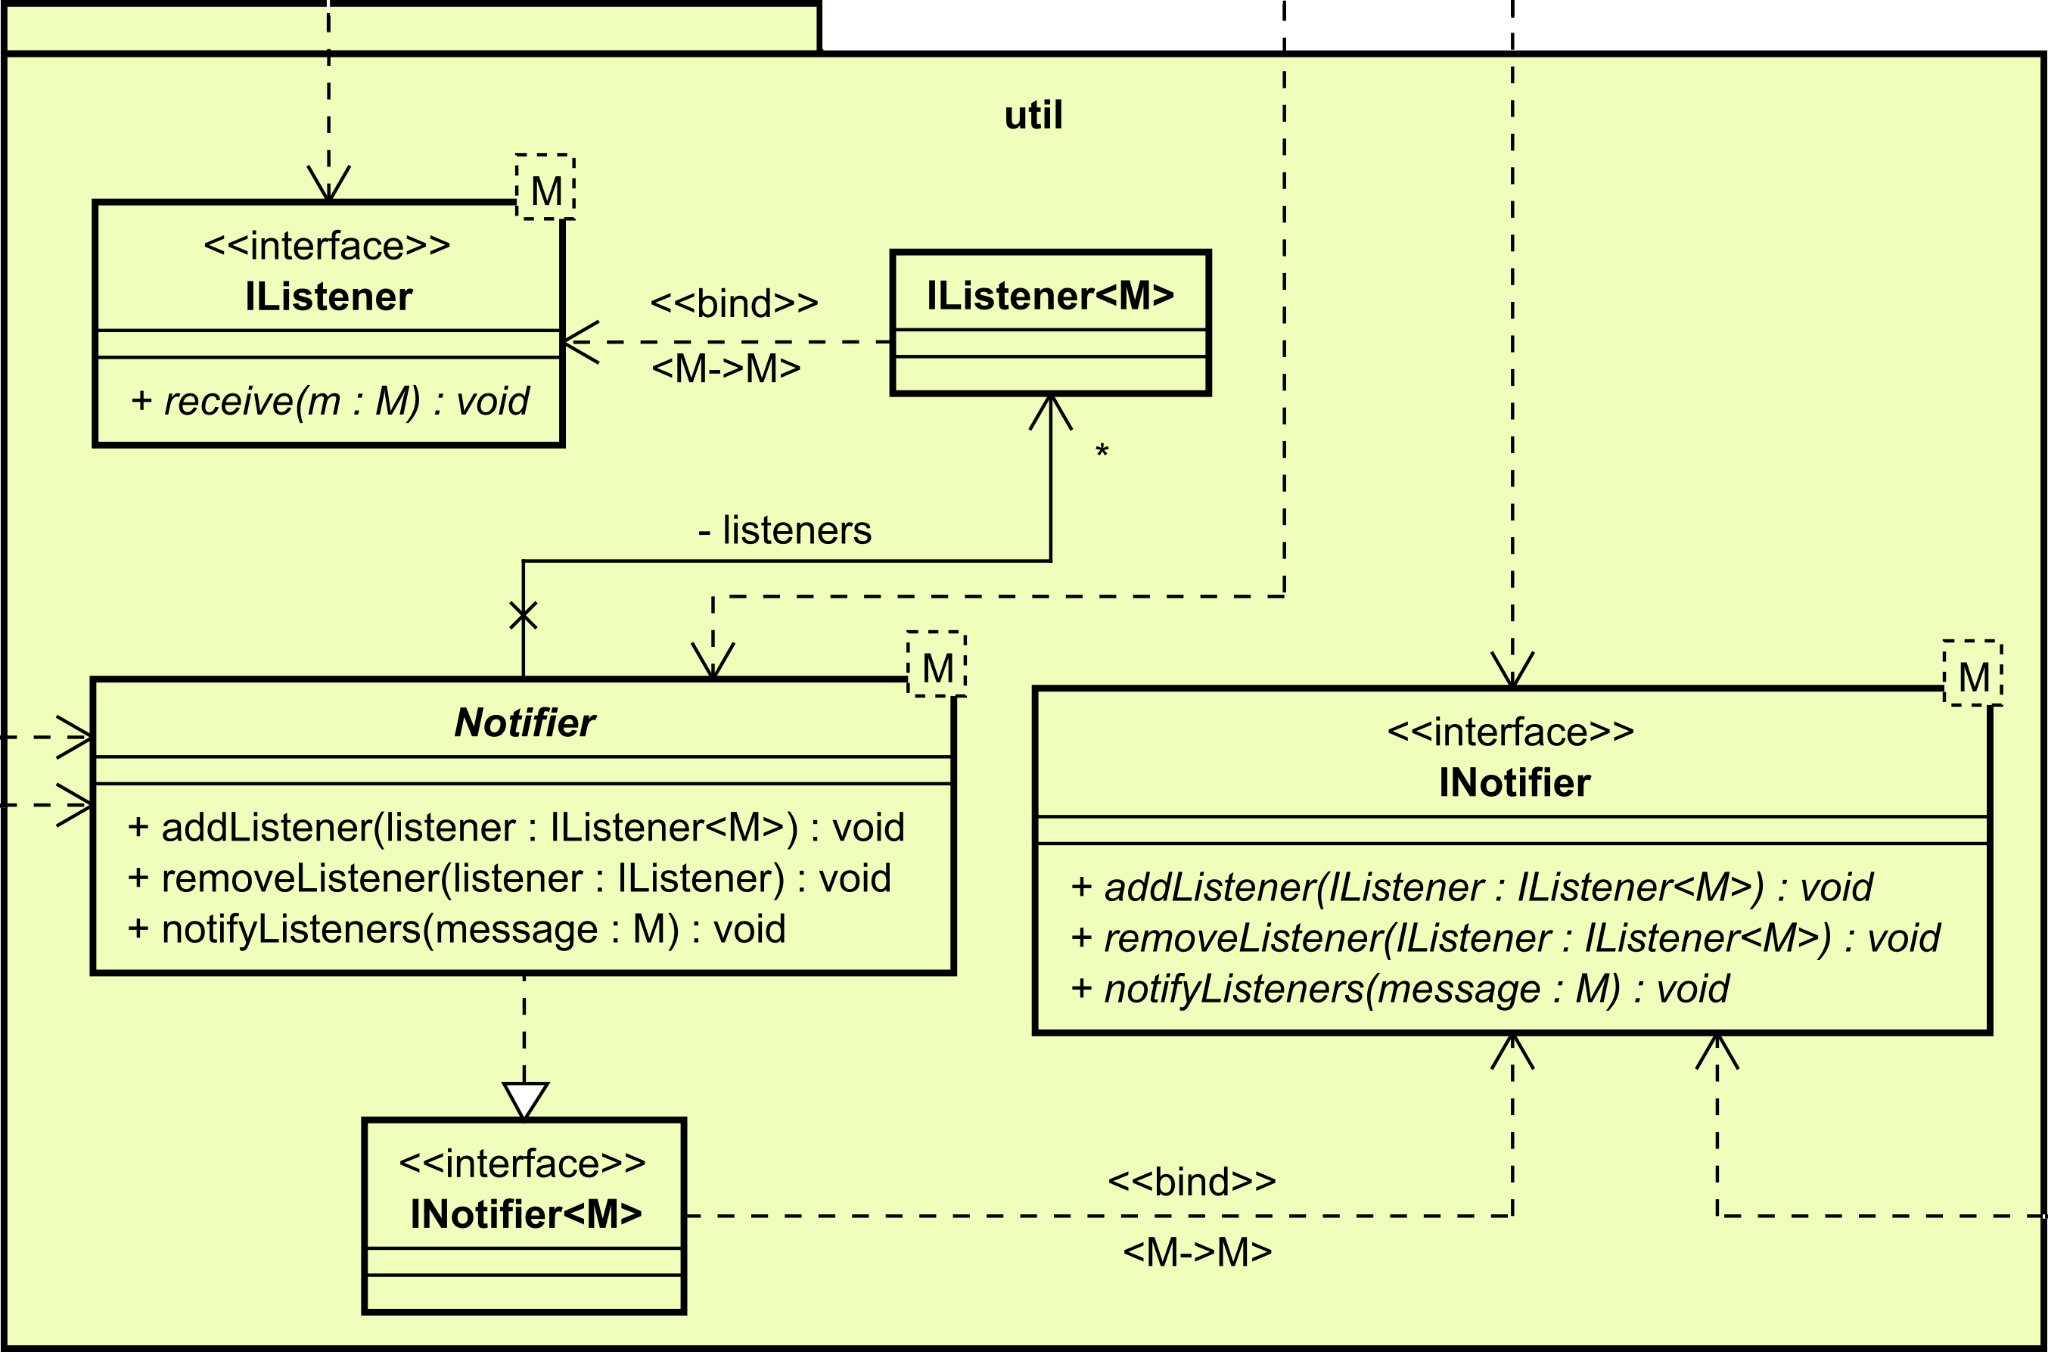
\includegraphics[width=\textwidth]{../diagramimages/util.png}
  \caption{\textbf{util-Package}}
\end{figure}

Da wir sowohl Interfaces als auch Klassen bzw. abstrakte Klassen als \gls{notifier} haben, kommen wir nicht um eine Modifizierung des klassischen \gls{observerpattern} herum. Nun haben wir die Möglichkeit sowohl ein \gls{notifier}-Interface zu erweitern als auch eine abstrakte \gls{notifier}-Klasse zu beerben. Der \gls{listener} funktioniert genau wie ein Observer.


\section{\textbf{model-Package:}}


Die Hauptdatenstruktur von \gls{programname}: das \textbf{model-Package}.

\begin{figure}[H]
  \centering
  \includegraphics[width=\textwidth]{../diagramimages/model.png}
  \caption{\textbf{model-Package}}
\end{figure}

    \subsection*{\textbf{graph}}
    
    \subsection*{\textbf{filter}}
    
    \subsection*{\textbf{settingsdata}}
    
    \subsection*{\textbf{graphlog}}


\section{\textbf{view-Package:}}


\section{\textbf{interactors-Package:}}


\chapter{Klassendokumentation}

\section{Service}

\subsection{TruffleReceiver}

\begin{figure}[h!]
    \centering
    \includegraphics[width=\textwidth]{../diagramimages/TruffleReceiver.png}
    \caption[Klasse TruffleReceiver]{Klasse TruffleReceiver}
    \medskip
    Diese Klasse empfängt ganz tolle Truffles und so ein zeug bla bla.
\end{figure}

\subsubsection*{Attribute}

\begin{easylist}[itemize]

    & Attribut 1

    & Attribut 2

\end{easylist}

\subsubsection*{Methoden}

\begin{easylist}[itemize]

    & Methode 1

    & Methode 2

\end{easylist} 

\chapter{Sequenzdiagramme}

\begin{figure}[H]
  \centering
  \includegraphics[width=\textwidth]{../diagramimages/spp-profinet-package-dissection.png}
  \caption[Sequenzdiagramm \sppname package dissection]{Sequenzdiagramm \sppname package dissection}
\end{figure}

In dieser Sequenz werden zwei zentrale Aufrufe von \gls{snort} im \gls{praeprozessor} \sppname dargestellt. Zum einen im oberen Teil die Initialisierung des \gls{praeprozessor}s durch einen Init-Aufruf, sowie der \gls{praeprozessor}-interne Aufbau des DecoderRegisters. Dieser Registrierungsvorgang wurde im Diagramm aus Platzgründen eingespaart. Darin wird jeder als C-Datei vorhandene Decoder instanziiert und bei der DecoderRegisterList registriert. Dieser Vorgang legt die Grundlage für den Decoder-Baum-Ablauf, welcher exemplarisch als zweiter unterer Teil des Sequenzdiagramms 

\chapter{Ressourcen}
\section{Dateien und Strukturen}
Im Folgenden ist das Datenhaltungsverzeichnis von \gls{programname} visualisiert. Alle persistenten, das heißt einen Neustart des Programms überdauernden Daten sind in Dateien in Unterordnern des Ordners \texttt{data} gespeichert.  
\begin{figure}[H]
  \centering
\begin{verbatim}
.
`-- data
    |-- config
    |   |-- filtermenu_en.properties
    |   |-- graphwindow_en.properties
    |   |-- logwindow_en.properties
    |   |-- notificationview_en.properties
    |   |-- settingsmenu_en.properties
    |   `-- statistics_en.properties
    |-- log
    |   `-- trufflehog.log
    |-- replay_log
    |   |-- graph_TIMESTAMP2.trufflesnapshot
    |   `-- graph_TIMESTAMP.trufflesnapshot
    `-- truffle_data_log
        |-- nodeA.xml
        `-- nodeB.xml
\end{verbatim}
  \caption[Ordner- und Dateiestruktur von \gls{programname}]{Ordner- und Dateiestruktur von \gls{programname}}
\end{figure}



\input{chapters/classindex}

\appendix

\printglossary[title=Glossar,toctitle=Glossar]

\end{document}
